\documentclass[11pt,a4paper]{article}

\usepackage[margin=1in]{geometry}
\usepackage{amsmath,amssymb}
\usepackage{booktabs}
\usepackage{pgfplots}
\pgfplotsset{compat=1.18}
\usepackage[round]{natbib}
\usepackage[colorlinks=true,linkcolor=black,citecolor=black,urlcolor=blue]{hyperref}
\usepackage{parskip}
\usepackage{caption}
\setlength{\emergencystretch}{1.5em}

\title{\textbf{Macro Regimes and a Concentrated Growth Fund}\\[0.4em]
\large Real-Time Evidence on Regime Timing versus Static Diversification, 1990--2026}
\author{Khanh Nguyen}
\date{}

\begin{document}
\maketitle

\begin{abstract}
\noindent Allocators often sort months into four macro regimes by the direction of growth and inflation and
change their holdings with the regime. We ask whether such a rule can protect a concentrated U.S.\ growth
fund, the JPMorgan Large Cap Growth Fund, without giving up its return. The regimes are built only from data
published at the time (766 vintages of industrial production and consumer prices that are never
revised), the fund's returns are checked against its annual report, and the overlay is tested under a
specification frozen before any backtest. Three results. First, revisions matter: real-time and revised
regimes agree in only $81.8\%$ of months, and the usual backtest construction agrees with what was
knowable in $67.3\%$. Second, real-time regimes do not forecast next month's excess return of any of
12 asset classes once 36 tests are accounted for, and for the growth fund the effect of
Stagflation reverses sign around 2007 ($+14.0\%$ a year relative to other regimes before, $-20.9\%$ after).
Third, a regime overlay improves the fund's Sharpe ratio from $0.75$ to $1.07$ in 2007--2026
(Ledoit--Wolf $p=$ $0.03$), with a timing component of $+0.22$ ($p=$ $0.07$); both gains rest on the
2008 crisis and are not significant without it. In 2000--2007 the same timing lowers the Sharpe ratio by
$-0.18$ (not significant), for the fund and for ten other equity funds and indices of different styles and
regions; these, however, behave like little more than one independent series. A standard predictive
regression on the same real-time signals has no out-of-sample skill and adds no value either, and the
stock--bond correlation does not explain the change. Holding the overlay's average weights without timing
reduces the drawdown in both periods and raises the Sharpe ratio over 2000--2026 ($+0.14$, 90\% interval
$[+0.05,\ +0.22]$). The robust recommendation is static diversification; regime timing is a bet on the post-2007 era.
\end{abstract}

%=====================================================================
\section{Introduction}
\label{sec:intro}

\paragraph{The problem.} Many investors hold a single concentrated growth fund. The JPMorgan Large Cap Growth
Fund is a good example: a large, well-run fund whose ten largest positions are about half of its assets and
which holds almost nothing outside U.S.\ growth equity. Its returns are excellent in most years, and its
drawdowns are deep when growth stocks fall together: $-47.6\%$ on month-end data in 2008 (Class I shares),
$-31.82\%$ from peak to trough in March 2020 on daily data, and $-27.81\%$ on month-end data in 2022. The
question is whether adding other assets, and changing how much is added with the macro environment, can keep
most of the return and cut those drawdowns.

\paragraph{Why macro regimes.} The idea that asset returns depend on the macro environment is old and
intuitive. Equities do well when growth rises and inflation falls; bonds do well when inflation falls;
commodities and gold are expected to help when inflation rises. Classifying each month by whether growth and
inflation are accelerating gives four regimes (Goldilocks, Reflation, Disinflation, Stagflation), and a
regime overlay holds the assets that historically did best in the current one. The framework is common in
practice \citep{ilmanen2011}; statistical versions with estimated regime probabilities have a long academic
history \citep{ang2002}.

\paragraph{Three ways such backtests go wrong.} First, macro data are revised. Industrial production is
published about two weeks after the month ends and then revised for years, so a backtest built on today's
data uses numbers nobody had \citep{croushore2001,orphanides2001}. Second, return predictability from macro
variables is fragile and often vanishes out of sample or across subperiods \citep{welch2008}. Third, an
allocation table chosen after trying many versions on the same data overstates what an investor would have
earned \citep{harvey2016,bailey2014}. A fourth, more mundane, problem is data: mutual-fund price series from
free vendors can mishandle distributions, which moves losses between months.

\paragraph{What this paper does.} We address each problem directly. Return data are checked against the
fund's annual report to the SEC. Regimes are built from the industrial production vintages published each
month and from consumer prices that are never revised, and a look-ahead test with a deliberate leak as a
positive control confirms that no decision uses later data. We then ask whether regimes forecast returns at
all, and finally test a specific overlay under a specification frozen before any backtest, against six simple
alternatives, in an earlier period that played no part in its design, and on ten other equity funds and
indices; we also test a standard predictive-regression alternative and one candidate mechanism.

\begin{table}[htbp]
\centering
\caption{Main results at a glance.}
\label{tab:glance}
\small
\begin{tabular}{@{}p{0.47\textwidth}p{0.45\textwidth}@{}}
\toprule
Question & Answer \\
\midrule
Do revisions change the regimes? & Real-time and revised regimes agree in $81.8\%$ of months \\
Do real-time regimes forecast next month's returns? & 0 of 36 tests pass a Bonferroni correction \\
Is the growth fund's Stagflation effect stable? & $+14.0\%$ a year before 2007, $-20.9\%$ after \\
Does the overlay's \emph{timing} add value, 2007--2026? & Sharpe $+0.22$, 90\% interval $[+0.03,\ +0.41]$; $+0.12$ without 2007-10 to 2009-03 \\
\quad and in 2000--2007? & Sharpe $-0.18$, 90\% interval $[-0.32,\ +0.05]$ \\
Does its \emph{average allocation} add value? & Sharpe $+0.09$ $[-0.01,\ +0.19]$ (2007--2026), $+0.22$ $[+0.11,\ +0.39]$ (2000--2007) \\
Same pattern for ten other equity assets? & Yes for all ten, but they behave like $1.2$ independent series \\
Does a predictive regression do better? & No: out-of-sample $R^2$ $-0.23\%$ and $-3.31\%$ \\
Does the stock--bond correlation explain the sign change? & No: within each period both states have the same sign \\
\bottomrule
\end{tabular}
\end{table}

\paragraph{Contributions.}
\begin{enumerate}
\item A real-time growth--inflation classifier and a measurement of what revisions change
(Section~\ref{sec:regimes}).
\item Evidence that regime-conditional returns are not a stable basis for allocation: no asset survives a
multiple-testing correction, and for growth equities the sign of the Stagflation effect reverses around 2007
(Section~\ref{sec:predict}).
\item A test of a regime overlay that separates static allocation from timing, uses an out-of-sample period
and hold-out assets, measures how independent those hold-outs are, and finds that the static part is robust and
the timing part is not (Sections~\ref{sec:design}--\ref{sec:results}). A standard predictive regression on the same
signals fails in the same way (Section~\ref{sec:model}).
\end{enumerate}

%=====================================================================
\section{Data and verification}
\label{sec:data}

\paragraph{Asset returns.} Daily total returns from Yahoo Finance, compounded to month-end, for the fund
(JLGMX, Class R6, from December 2010; before that its Class I shares SEEGX, the same portfolio with returns
$0.31$ points a year lower on average because of the higher fee), growth and broad equity benchmarks,
three other growth funds, and eight non-equity ETFs. Excess returns are over the 3-month Treasury bill. Before
the ETFs exist, long-history proxies are used (Appendix~\ref{app:proxy}).

\paragraph{Verification.} A single vendor is a single point of failure, so we checked the data against an
independent source: the fund's annual report to the SEC, which states average annual total returns to 30
June 2026 (Table~\ref{tab:data}).

\begin{table}[htbp]
\centering
\caption{Average annual total returns to 2026-06-30 (\%): computed from our data vs.\ the annual report (or,
for IWF, the index it tracks, before its $0.19\%$ fee).}
\label{tab:data}
\small
\begin{tabular}{@{}lrrrrrr@{}}
\toprule
& \multicolumn{2}{c}{1 year} & \multicolumn{2}{c}{5 years} & \multicolumn{2}{c}{10 years} \\
\cmidrule(lr){2-3}\cmidrule(lr){4-5}\cmidrule(lr){6-7}
& Ours & Report & Ours & Report & Ours & Report \\
\midrule
JLGMX (Class R6) & $15.53$ & $15.56$ & $12.60$ & $12.66$ & $20.29$ & $20.30$ \\
SEEGX (Class I) & $15.23$ & $15.26$ & $12.31$ & $12.38$ & $19.98$ & $19.99$ \\
IWF vs.\ Russell 1000 Growth & $17.41$ & $17.71$ & $13.51$ & $13.71$ & $18.36$ & $18.58$ \\
\bottomrule
\end{tabular}
\end{table}

The fund numbers agree to within $0.07$ percentage points a year. Three further checks: adjusted prices
equal raw prices plus reinvested distributions on at least $99.7\%$ of days for every series; the two share
classes differ by $0.20$ to $0.38$ points a year, which is their fee difference, and never by more than
$0.07$ points in a month; and no fund shows a drop of more than 4\% on a day when the market moved
less than 1.5\%, the signature of a missing distribution.

\paragraph{Why this matters: an earlier backtest.} An earlier backtest of the overlay studied here, run by the
author on vendor monthly prices for 2011--2026, is a useful warning (Table~\ref{tab:old}). Its compound
return for the fund is the same as ours, $16.8\%$, but its volatility was $4.1$ percentage
points higher and its losses were placed in the wrong months: $-29\%$ in late 2018 that was really $-18.5\%$,
and $-13\%$ in 2022 that was really $-23.4\%$. The same compound return with more volatility is the signature
of distributions recorded in the wrong month: a fund that pays a large capital gain in December shows a fake
drop when the payment is missed and a fake recovery when it is caught up. On those data the overlay appeared
to raise the return ($16.81\%$ against $16.49\%$); on verified data it lowers it
($14.69\%$ against $16.81\%$).

\begin{table}[htbp]
\centering
\caption{The earlier backtest on vendor monthly prices against verified data, 2011-02 to 2026-05. Sharpe
here is (CAGR $-$ T-bill)/volatility, the convention of the earlier backtest. K is the overlay of
Section~\ref{sec:design}; on verified data it uses the real-time classifier.}
\label{tab:old}
\small
\begin{tabular}{@{}lrr@{}}
\toprule
& Earlier backtest & Verified data \\
\midrule
Fund, Oct--Dec 2018 & $-29.07\%$ & $-18.52\%$ \\
Fund, Feb--Mar 2020 & $-14.88\%$ & $-14.88\%$ \\
Fund, Jan--Oct 2022 & $-12.56\%$ & $-23.37\%$ \\
Fund, CAGR 2011-02 to 2026-05 & $16.81\%$ & $16.81\%$ \\
Fund, volatility & $20.73\%$ & $16.65\%$ \\
Fund, Sharpe (old convention) & $0.74$ & $0.92$ \\
Fund, maximum drawdown & $-29.07\%$ & $-27.81\%$ \\
\midrule
K, CAGR & $17.05\%$ & $14.69\%$ \\
K, volatility & $15.28\%$ & $11.54\%$ \\
K, Sharpe (old convention) & $1.01$ & $1.14$ \\
K, maximum drawdown & $-13.41\%$ & $-17.60\%$ \\
\bottomrule
\end{tabular}
\end{table}

\paragraph{Macro data.} The Real-Time Data Set for Macroeconomists of the Federal Reserve Bank of
Philadelphia \citep{croushore2001} records, for each month from 1962-11 to 2026-08, the history of
industrial production as published in the middle of that month: 766 vintages. Each vintage ends with the
previous month, except the October and November 2025 vintages, which end in August 2025 because the federal
shutdown delayed the release. The last vintage matches today's FRED series to within $0.33\%$. For
inflation we use the consumer price index \emph{not} seasonally adjusted, which is never revised; its
year-on-year change correlates $0.9992$ with that of the adjusted index and never differs by more than
$0.27$ points.

%=====================================================================
\section{Regimes in real time}
\label{sec:regimes}

\paragraph{Timing.} The decision is made at the end of month $t$ and applies to returns in month $t+1$. At that
moment industrial production is known through month $t-1$ (the vintage dated $t$), and so are consumer
prices.

\paragraph{Signals and regimes.} For each series we take the year-on-year growth rate and its change over six
months, $d_t = \text{YoY}_{t-1} - \text{YoY}_{t-7}$, computed within the vintage available at $t$. Year-on-year
growth removes seasonality; the six-month change asks whether conditions are improving or worsening.
Goldilocks: growth up, inflation down. Reflation: both up. Disinflation: both down. Stagflation: growth down,
inflation up.

\paragraph{Variants.} The raw classifier uses the signals as they are. A smoothed version averages each signal
over three months, and a persistent version changes regime only after a new label has appeared for three
consecutive months. For comparison we also build the classifier as it is usually backtested: today's revised
industrial production, seasonally adjusted prices and a fixed lag.

\paragraph{Look-ahead test.} We delete every input published after month $t$, rerun the classifier, and compare
every label up to $t$ with the full-data run. At 60 randomly chosen months the labels are identical in
60 of 60 cases. A test that never fails proves little, so we also ran it after letting the next
month's prices leak into the signal: it flagged 60 of 60 cuts.

\begin{table}[htbp]
\centering
\caption{Regime statistics, decisions 1990--2026. Switches: regime changes; spell: average months per
regime; last four columns: share of months in each regime.}
\label{tab:spells}
\small
\begin{tabular}{@{}lrrrrrrr@{}}
\toprule
Classifier & Months & Switches & Spell & Gold. & Refl. & Disinf. & Stagf. \\
\midrule
Real time, raw & 440 & 122 & $3.6$ & $21\%$ & $30\%$ & $27\%$ & $22\%$ \\
Real time, smoothed & 438 & 94 & $4.6$ & $20\%$ & $30\%$ & $28\%$ & $21\%$ \\
Real time, smoothed + persistent & 438 & 58 & $7.4$ & $20\%$ & $32\%$ & $28\%$ & $20\%$ \\
Revised, lag 1 & 440 & 137 & $3.2$ & $21\%$ & $30\%$ & $26\%$ & $23\%$ \\
Revised, lag 2 & 440 & 137 & $3.2$ & $21\%$ & $30\%$ & $26\%$ & $23\%$ \\
Revised, lag 2, smoothed + persistent & 439 & 57 & $7.6$ & $18\%$ & $30\%$ & $32\%$ & $20\%$ \\
\bottomrule
\end{tabular}
\end{table}

\paragraph{What revisions change.} Under the same rules and lag, real-time and revised classifiers agree in
$81.8\%$ of months. The difference comes from growth: the sign of the growth signal agrees in
$83.6\%$ of months (correlation $0.957$), that of the inflation signal in $97.7\%$ (correlation
$0.997$). The usual construction, revised data with a two-month lag, agrees with the real-time labels in
only $67.3\%$ of months: roughly $33\%$ of the labels in such a backtest could not have been
known when the trade was made. Smoothing does not wash this out (agreement $70.1\%$), because the
persistence rule turns a small change in timing into a different regime for several months.

\paragraph{Stability.} The raw classifier switches 122 times in 440 months, every
$3.6$ months on average (Table~\ref{tab:spells}); smoothing and persistence reduce this to
58 switches at the cost of reacting later. Delaying the raw classifier by one, two or three further
months leaves only $72.3\%$, $56.1\%$ and $45.2\%$ of labels unchanged.

\begin{table}[htbp]
\centering
\caption{The 2008 crisis month by month. ``IP through'': last month of industrial production available at the
decision; $d^g$, $d^\pi$: real-time growth and inflation signals (percentage points).}
\label{tab:2008}
\footnotesize
\setlength{\tabcolsep}{4pt}
\begin{tabular}{@{}llrrlll@{}}
\toprule
Decision & IP through & $d^g$ & $d^\pi$ & Real time, raw & Real time, persistent & Revised, lag 2 \\
\midrule
2007-10 & 2007-09 & $-0.22$ & $-0.02$ & Disinflation & Stagflation & Disinflation \\
2007-11 & 2007-10 & $-0.20$ & $+0.96$ & Stagflation & Stagflation & Reflation \\
2007-12 & 2007-11 & $+0.26$ & $+1.62$ & Reflation & Stagflation & Stagflation \\
2008-01 & 2007-12 & $+0.17$ & $+1.39$ & Reflation & Stagflation & Reflation \\
2008-02 & 2008-01 & $+0.55$ & $+1.92$ & Reflation & Stagflation & Stagflation \\
2008-03 & 2008-02 & $-0.36$ & $+2.06$ & Stagflation & Reflation & Stagflation \\
2008-04 & 2008-03 & $-0.74$ & $+1.23$ & Stagflation & Reflation & Stagflation \\
2008-05 & 2008-04 & $-1.73$ & $+0.40$ & Stagflation & Reflation & Stagflation \\
2008-06 & 2008-05 & $-2.65$ & $-0.13$ & Disinflation & Stagflation & Stagflation \\
2008-07 & 2008-06 & $-1.73$ & $+0.94$ & Stagflation & Stagflation & Disinflation \\
2008-08 & 2008-07 & $-2.73$ & $+1.32$ & Stagflation & Stagflation & Stagflation \\
2008-09 & 2008-08 & $-3.15$ & $+1.35$ & Stagflation & Stagflation & Stagflation \\
2008-10 & 2008-09 & $-5.90$ & $+0.96$ & Stagflation & Stagflation & Stagflation \\
2008-11 & 2008-10 & $-4.39$ & $-0.28$ & Disinflation & Stagflation & Stagflation \\
2008-12 & 2008-11 & $-5.70$ & $-3.11$ & Disinflation & Stagflation & Disinflation \\
2009-01 & 2008-12 & $-7.74$ & $-4.93$ & Disinflation & Stagflation & Disinflation \\
2009-02 & 2009-01 & $-9.32$ & $-5.57$ & Disinflation & Disinflation & Disinflation \\
2009-03 & 2009-02 & $-9.26$ & $-5.14$ & Disinflation & Disinflation & Disinflation \\
\bottomrule
\end{tabular}
\end{table}

\paragraph{An example.} In real time the inflation signal stayed positive into the autumn of 2008 because
energy prices rose until July, while growth was already falling (Table~\ref{tab:2008}). The raw classifier
labels most of 2008 Stagflation and switches to Disinflation in November; the persistent version keeps
Stagflation until early 2009; the revised version moves between regimes in a different order. For an
allocation rule the differences are large: the same month can call for 25\% or 80\% in equities depending on
which version is used.

%=====================================================================
\section{Do regimes forecast returns?}
\label{sec:predict}

\paragraph{Test.} For each asset we regress the excess return of month $t+1$ on four dummies for the regime known
at the end of month $t$; the coefficients are the average excess returns by regime. Standard errors are
Newey--West with six lags \citep{newey1987}. A Wald test asks whether the four means are equal, and a contrast
measures Stagflation minus the average of the other regimes, the comparison regime-based de-risking relies on.
With 12 assets and three classifiers there are 36 tests, so a Bonferroni correction requires
$p<$ $0.0014$.

\begin{table}[htbp]
\centering
\caption{Wald $p$-values for equal mean excess returns across regimes, from the date shown to 2026-09; last two
columns: Stagflation minus the other regimes (\%/yr) and its $t$-statistic, real-time raw classifier.}
\label{tab:wald}
\footnotesize
\setlength{\tabcolsep}{4pt}
\begin{tabular}{@{}lrrrrrr@{}}
\toprule
& & \multicolumn{3}{c}{Wald $p$} & \multicolumn{2}{c}{Stagflation $-$ others} \\
\cmidrule(lr){3-5}\cmidrule(lr){6-7}
Asset & From & Real time & RT persistent & Revised & \%/yr & $t$ \\
\midrule
Large Cap Growth (SEEGX) & 1992-03 & $0.501$ & $0.705$ & $0.522$ & $-6.9$ & $-0.90$ \\
S\&P 500 (SPY) & 1993-02 & $0.590$ & $0.402$ & $0.740$ & $-3.8$ & $-0.54$ \\
Russell 1000 Growth (IWF) & 2000-06 & $0.374$ & $0.683$ & $0.217$ & $-9.5$ & $-1.20$ \\
Nasdaq-100 (QQQ) & 1999-04 & $0.459$ & $0.739$ & $0.360$ & $-11.6$ & $-1.27$ \\
7--10y Treasuries (IEF) & 2002-08 & $0.406$ & $0.985$ & $0.423$ & $+5.1$ & $+1.53$ \\
20y+ Treasuries (TLT) & 2002-08 & $0.185$ & $0.932$ & $0.498$ & $+13.2$ & $+1.91$ \\
1--3y Treasuries (SHY) & 2002-08 & $0.930$ & $0.276$ & $0.240$ & $+0.5$ & $+0.58$ \\
TIPS (TIP) & 2004-01 & $0.605$ & $0.989$ & $0.464$ & $-0.7$ & $-0.21$ \\
Gold (GLD) & 2004-12 & $0.262$ & $0.138$ & $0.808$ & $+2.4$ & $+0.33$ \\
High yield (HYG) & 2007-05 & $0.021$ & $0.830$ & $0.153$ & $-12.2$ & $-1.65$ \\
US dollar (UUP) & 2007-04 & $0.055$ & $0.549$ & $0.588$ & $+4.1$ & $+1.02$ \\
Commodities (DBC) & 2006-03 & $0.172$ & $0.487$ & $0.331$ & $-10.8$ & $-0.73$ \\
\bottomrule
\end{tabular}
\end{table}

\paragraph{No asset survives.} With the real-time raw classifier 1 of 12 assets has $p<0.05$
(high yield, $p=$ $0.021$), and 0 of the 36 tests pass the Bonferroni level
(Table~\ref{tab:wald}). Point estimates are often large: long Treasuries earn $+12.7\%$ a year more in
Stagflation ($t=$ $2.01$), and gold earns $+12.4\%$ in Stagflation but also $+21.4\%$ in
Goldilocks. Monthly returns are too noisy, and regime episodes too few, to separate these from chance.

The long-Treasury estimate contradicts a popular rule. Many regime allocations exclude long bonds in
Stagflation because of 2022, when stocks and bonds fell together. In real time only 4 return months
of 2022 follow a Stagflation label, and in them long Treasuries returned $-52\%$ a year. Among years with
at least four such months, the four best for long Treasuries were 2020 (4 months, $+65\%$), 2011 (11 months, $+37\%$), 2016 (6 months, $+31\%$), 2008 (7 months, $+23\%$); excluding 2008 they still earn
$+11.6\%$ a year in Stagflation. A rule drawn from one episode does not describe the regime.

\begin{table}[htbp]
\centering
\caption{The growth fund (SEEGX) by real-time regime: months, annualised excess return (\%) and Sharpe ratio,
over the full sample and before and after March 2007.}
\label{tab:fund}
\footnotesize
\setlength{\tabcolsep}{3.5pt}
\begin{tabular}{@{}lrrrrrrrrr@{}}
\toprule
& \multicolumn{3}{c}{1992--2026} & \multicolumn{3}{c}{1992--2007} & \multicolumn{3}{c}{2007--2026} \\
\cmidrule(lr){2-4}\cmidrule(lr){5-7}\cmidrule(lr){8-10}
Regime & $n$ & Excess & SR & $n$ & Excess & SR & $n$ & Excess & SR \\
\midrule
Goldilocks & 84 & $+15.8$ & $+1.05$ & 40 & $+1.1$ & $+0.08$ & 44 & $+29.2$ & $+2.05$ \\
Reflation & 130 & $+6.4$ & $+0.39$ & 63 & $+7.2$ & $+0.47$ & 67 & $+5.6$ & $+0.32$ \\
Disinflation & 111 & $+12.2$ & $+0.71$ & 46 & $-3.2$ & $-0.18$ & 65 & $+23.0$ & $+1.38$ \\
Stagflation & 90 & $+4.6$ & $+0.24$ & 32 & $+15.8$ & $+1.00$ & 58 & $-1.6$ & $-0.08$ \\
\midrule Wald $p$ (equal means) & \multicolumn{3}{c}{$0.501$} & \multicolumn{3}{c}{$0.367$} & \multicolumn{3}{c}{$0.004$} \\
Stagflation $-$ others (\%/yr) & \multicolumn{3}{c}{$-6.9$ ($t=-0.90$)} & \multicolumn{3}{c}{$+14.0$ ($t=1.36$)} & \multicolumn{3}{c}{$-20.9$ ($t=-2.21$)} \\
\bottomrule
\end{tabular}
\end{table}

\begin{figure}[htbp]
\centering
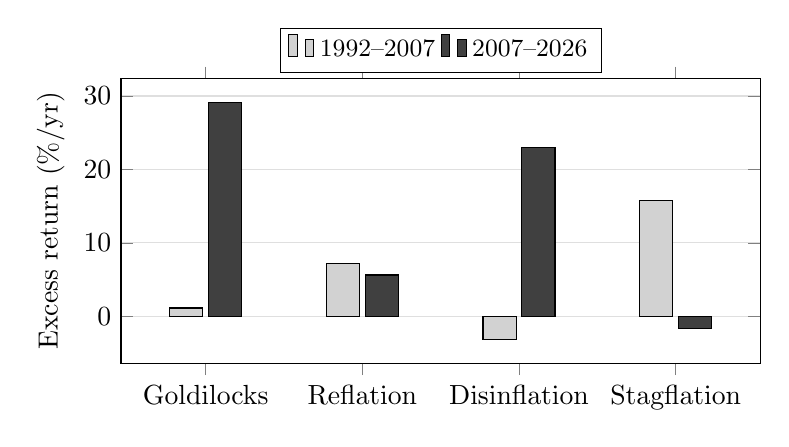
\begin{tikzpicture}
\begin{axis}[ybar, bar width=12pt, width=0.8\textwidth, height=5.2cm, symbolic x coords={Goldilocks,Reflation,Disinflation,Stagflation},
  xtick=data, ylabel={Excess return (\%/yr)}, legend style={at={(0.5,1.02)},anchor=south,legend columns=2,font=\small},
  ymajorgrids, grid style={gray!25}, enlarge x limits=0.18]
\addplot[fill=gray!35, draw=black] coordinates {(Goldilocks,1.13) (Reflation,7.20) (Disinflation,-3.16) (Stagflation,15.77)}; \addlegendentry{1992--2007}
\addplot[fill=black!75, draw=black] coordinates {(Goldilocks,29.17) (Reflation,5.62) (Disinflation,22.98) (Stagflation,-1.63)}; \addlegendentry{2007--2026}
\end{axis}
\end{tikzpicture}
\caption{Annualised excess return of the growth fund in the month after each real-time regime.}
\label{fig:fund}
\end{figure}

\paragraph{The growth fund: the sign changes.} Over the full sample the fund earns $+4.6\%$ a year above bills
after Stagflation months, and the contrast with other regimes is $-6.9\%$ ($t=$ $-0.90$). The two halves of
the sample disagree (Table~\ref{tab:fund}, Figure~\ref{fig:fund}). Before 2007, Stagflation was the fund's
\emph{best} regime ($+15.8\%$, contrast $+14.0\%$); after 2007 it was close to its worst ($-1.6\%$,
contrast $-20.9\%$, $t=$ $-2.21$, Wald $p=$ $0.004$). The pre-2007 contrast alone is not significant
($t=$ $+1.36$), but the change between the periods is: $34.9$ points a year, $z=$ $2.50$, $p=$ $0.01$
(the periods do not overlap; the split is the start of the joint ETF sample, fixed before any regime result). After 2007 the regime means also differ
significantly for SEEGX, SPY, IWF, QQQ, HYG; before 2007 none of the 4 assets with enough history shows a
significant difference. Even after 2007 the result depends on the classifier: with the persistent version the
fund's Wald $p$ is $0.54$.

\paragraph{Why the sign might change.} Stagflation decision months are spread over 14 calendar
years before 2007 and 14 after; the largest clusters are 2005 (7), 1990 (5), 1998 (4), 1992 (3) before and
2011 (11), 2008 (7), 2007 (6), 2013 (5) after. The second half contains the 2008 crash (13 Stagflation months in
2007--2008); the 2022 inflation shock contributes only 3, because year-on-year growth of industrial
production was still rising in the decisions from March to August 2022. \citet{campbell2020} link the change in
sign of the stock--bond correlation around 2000 to changes in monetary policy and in the nature of inflation
shocks; a similar change could make the equity response to rising inflation depend on the era. This is a
hypothesis; the data cannot separate it from the simpler explanation that a few episodes dominate each half.

\paragraph{Testing that mechanism.} We can test one version directly. At each decision month we compute the
correlation between the fund's and intermediate Treasuries' monthly returns over the previous 36 months, which is
known at the time, and let the regime effect differ by its sign (decisions from 1995-02). Over the full sample
the direction is as the hypothesis predicts: the Stagflation contrast is $+2.1\%$ a year when the correlation is
positive ($t=$ $0.16$) and $-12.0\%$ when it is negative ($t=$ $-1.25$). But the difference is far from
significant ($t=$ $0.86$), and within each period both states have the same sign: $+20.5\%$ and
$+12.0\%$ before 2007, $-10.9\%$ and $-24.4\%$ after. The correlation was positive in
$48\%$ of months before 2007 and $29\%$ after, so it moves with the era, but it does not explain the
sign change: the change follows the calendar, not the correlation state.

\paragraph{Power.} The standard error of the fund's Stagflation contrast is $7.7\%$ a year, so an effect would
have to be about $21\%$ a year to be detected with 80\% probability at the 5\% level ($29\%$ and
$26\%$ in the two halves). The data do not show that regimes are irrelevant. They show that differences of
the size observed cannot be told from chance and do not keep their sign, which is a weak basis for an
allocation rule.

%=====================================================================
\section{The overlay and the test design}
\label{sec:design}

\begin{table}[htbp]
\centering
\caption{Overlay K: weights (\%) by regime, frozen before this study.}
\label{tab:k}
\small
\begin{tabular}{@{}lrrrrrr@{}}
\toprule
Regime (growth, inflation) & Fund & High yield & Gold & Commodities & 1--3y Treasuries & Dollar \\
\midrule
Goldilocks (up, down) & 90 & 10 & & & & \\
Reflation (up, up) & 55 & 10 & 30 & 5 & & \\
Disinflation (down, down) & 80 & 10 & 10 & & & \\
Stagflation (down, up) & 25 & & 25 & & 30 & 20 \\
\bottomrule
\end{tabular}
\end{table}

\paragraph{The overlay.} Overlay K (Table~\ref{tab:k}) is a typical regime table. It keeps most of the fund in
Goldilocks and Disinflation, cuts it deeply in Stagflation, and chooses hedges by regime: gold and
commodities when inflation rises, short Treasuries and dollars in Stagflation, and a high-yield sleeve when
growth rises. It was chosen by the author in the earlier backtest of Section~\ref{sec:data}, on 2011--2026
data, after trying about 40 configurations, and motivated by regime averages and by 2022. It is
therefore treated here as a hypothesis, frozen exactly as it was, and tested under conditions it was not
designed for.

\paragraph{Specification frozen before any backtest.} Every choice below was written down before the first
backtest was run.
\begin{itemize}
\item \textbf{Regimes:} the real-time raw classifier of Section~\ref{sec:regimes}; the smoothed persistent and
revised versions are sensitivity checks.
\item \textbf{Rebalancing and costs:} monthly to target weights; turnover measured against the weights after the
previous month's drift; one-way costs of 1--5 basis points per unit of turnover depending on the ETF, zero for
the fund.
\item \textbf{Periods:} 2007-04 to 2026-09, when every ETF exists, containing 2008, 2020 and 2022; and 2000-10 to
2007-03, which contains the dot-com crash and played no part in designing K (sleeves before ETF inception use
the proxies of Appendix~\ref{app:proxy}; gold futures start in August 2000).
\end{itemize}

\paragraph{Alternatives.} Each answers a specific question.
\begin{itemize}
\item \textbf{S-K}, the static mix with K's average weights over the same period: does K's \emph{timing} add
anything beyond its average allocation? Over 2007--2026 these weights are fund 61\%, HYG 8\%, GLD 18\%, DBC 1\%, SHY 7\%, UUP 5\%. S-K is an attribution
benchmark, not an investable strategy, because its weights use each period's regime frequencies. The fund weight
is similar in the two periods ($61\%$ after 2007, $64\%$ before), so a static mix fixed in advance would
have been close to it.
\item \textbf{G}, generic de-risking: 100\% fund in Goldilocks, otherwise 70\% fund, 15\% short Treasuries and 15\%
gold. Does choosing different hedges in different regimes matter?
\item \textbf{60/40} fund and intermediate Treasuries: the textbook balanced portfolio.
\item \textbf{Volatility target}: fund weight $\min(1,\ 15\%/\hat\sigma)$ with $\hat\sigma$ the trailing 12-month
volatility, the rest in short Treasuries \citep{moreira2017}.
\item \textbf{10-month trend}: the fund when its total-return index is above its 10-month average, otherwise short
Treasuries \citep{faber2007,moskowitz2012}.
\item \textbf{90/10} fund and gold: the simplest permanent hedge.
\end{itemize}

\paragraph{Attribution.} K minus fund $=$ (S-K minus fund) $+$ (K minus S-K): what the average allocation
contributes plus what timing contributes, applied to the Sharpe ratio, the maximum drawdown and the average
return.

\paragraph{Statistics.} Differences in Sharpe ratio and drawdown are resampled with the stationary bootstrap
\citep{politis1994} (mean block 12 months, 5{,}000 draws, all strategies on the same resampled months), a
bootstrap version of the test of \citet{ledoit2008}.

\paragraph{Success criterion.} Regime timing adds value only if the 90\% interval of Sharpe(K) $-$ Sharpe(S-K) is
above zero in both periods, and at least five of six other funds show a positive difference in both periods.
The criterion was written after the tests of Section~\ref{sec:predict}, which had shown that the fund's
returns by regime differ before and after 2007; a reader may regard the earlier period's result as partly
anticipated. Section~\ref{sec:where} shows that the loss there came mainly from regimes other than Stagflation.

\paragraph{Checks of the code.} A 100\% fund strategy reproduces the fund's returns exactly; turnover and costs
match a hand computation; K's weights match the table every month; the volatility and trend weights do not
change when later returns are deleted, while a version that peeks one month ahead is flagged by the same test
(8 of 18 cuts); 21 of 21 regression checks pass; and two full runs from raw data give
identical output.

%=====================================================================
\section{Results}
\label{sec:results}

\begin{table}[htbp]
\centering
\caption{2007-04 to 2026-09, real-time classifier, after costs. Worst 12m: worst 12-month return; Fund wt.:
average weight in the fund; Turn.: turnover per year.}
\label{tab:p1}
\small
\setlength{\tabcolsep}{4pt}
\begin{tabular}{@{}lrrrrrrr@{}}
\toprule
Strategy & CAGR & Vol. & Sharpe & Max DD & Worst 12m & Fund wt. & Turn. \\
\midrule
K (regime table) & $14.3\%$ & $11.9\%$ & $1.07$ & $-18.2\%$ & $-17.6\%$ & $0.61$ & $2.94$ \\
G (generic de-risking) & $13.1\%$ & $13.6\%$ & $0.87$ & $-33.0\%$ & $-28.2\%$ & $0.76$ & $1.39$ \\
Fund & $14.1\%$ & $17.7\%$ & $0.75$ & $-47.6\%$ & $-39.8\%$ & $1.00$ & $0.05$ \\
S-K (static K weights) & $11.4\%$ & $11.9\%$ & $0.84$ & $-31.0\%$ & $-26.6\%$ & $0.61$ & $0.32$ \\
60/40 fund/IEF & $10.0\%$ & $10.8\%$ & $0.80$ & $-27.0\%$ & $-22.3\%$ & $0.60$ & $0.30$ \\
Volatility target 15\% & $11.7\%$ & $15.1\%$ & $0.72$ & $-36.1\%$ & $-29.7\%$ & $0.87$ & $0.73$ \\
10-month trend & $11.4\%$ & $13.7\%$ & $0.76$ & $-19.7\%$ & $-18.4\%$ & $0.79$ & $3.74$ \\
90/10 fund/GLD & $13.9\%$ & $16.2\%$ & $0.80$ & $-42.6\%$ & $-35.9\%$ & $0.90$ & $0.17$ \\
\bottomrule
\end{tabular}
\end{table}

\paragraph{2007--2026 (Table~\ref{tab:p1}).} The fund returns $14.1\%$ a year with a volatility of
$17.7\%$ and a maximum drawdown of $-47.6\%$, in 2008. K keeps the return ($14.3\%$) with $0.67$
times the volatility, and its worst drawdown is $-18.2\%$: its Sharpe ratio is $1.07$ against $0.75$.
The static mix S-K has a similar volatility ($11.9\%$) but a lower return ($11.4\%$) and a much deeper
drawdown ($-31.0\%$), so timing explains most of K's advantage here. The 10-month trend rule matches K's
drawdown ($-19.7\%$) but not its Sharpe ratio ($0.76$).

\begin{table}[htbp]
\centering
\caption{2000-10 to 2007-03, real-time classifier, after costs; sleeves before ETF inception use proxies.}
\label{tab:p0}
\small
\setlength{\tabcolsep}{4pt}
\begin{tabular}{@{}lrrrrrrr@{}}
\toprule
Strategy & CAGR & Vol. & Sharpe & Max DD & Worst 12m & Fund wt. & Turn. \\
\midrule
K (regime table) & $-2.2\%$ & $11.9\%$ & $-0.35$ & $-47.5\%$ & $-36.5\%$ & $0.64$ & $4.03$ \\
G (generic de-risking) & $-2.9\%$ & $12.9\%$ & $-0.37$ & $-48.2\%$ & $-33.8\%$ & $0.77$ & $1.25$ \\
Fund & $-5.2\%$ & $16.7\%$ & $-0.40$ & $-56.8\%$ & $-43.5\%$ & $1.00$ & $0.15$ \\
S-K (static K weights) & $0.2\%$ & $10.9\%$ & $-0.18$ & $-38.1\%$ & $-28.7\%$ & $0.64$ & $0.41$ \\
60/40 fund/IEF & $-0.1\%$ & $9.3\%$ & $-0.26$ & $-31.3\%$ & $-23.8\%$ & $0.60$ & $0.41$ \\
Volatility target 15\% & $-0.4\%$ & $11.7\%$ & $-0.21$ & $-37.3\%$ & $-23.9\%$ & $0.84$ & $0.60$ \\
10-month trend & $7.4\%$ & $6.2\%$ & $0.73$ & $-7.4\%$ & $-6.0\%$ & $0.47$ & $2.31$ \\
90/10 fund/GLD & $-3.1\%$ & $15.0\%$ & $-0.32$ & $-51.8\%$ & $-39.5\%$ & $0.90$ & $0.27$ \\
\bottomrule
\end{tabular}
\end{table}

\paragraph{2000--2007, out of sample (Table~\ref{tab:p0}).} The period starts near the top of the technology bubble;
the fund loses $-5.2\%$ a year with a drawdown of $-56.8\%$. K loses less ($-2.2\%$, drawdown
$-47.5\%$), but its static mix does better still ($0.2\%$, drawdown $-38.1\%$): here K's timing made
things worse. The trend rule is the clear winner ($7.4\%$ a year, drawdown $-7.4\%$); its average fund
weight from October 2000 to December 2002 was $0\%$, so it sat out the decline.

\begin{table}[htbp]
\centering
\caption{Attribution of K minus fund into static allocation (S-K minus fund) and timing (K minus S-K). Sharpe
ratio; maximum drawdown in percentage points (positive = shallower); arithmetic return in points a year.}
\label{tab:attr}
\footnotesize
\setlength{\tabcolsep}{4pt}
\begin{tabular}{@{}llrrrrrr@{}}
\toprule
& & \multicolumn{2}{c}{Sharpe} & \multicolumn{2}{c}{Max DD (pp)} & \multicolumn{2}{c}{Return (pp/yr)} \\
\cmidrule(lr){3-4}\cmidrule(lr){5-6}\cmidrule(lr){7-8}
Classifier & Period & Static & Timing & Static & Timing & Static & Timing \\
\midrule
Real time, raw & 2007--2026 & $+0.09$ & $+0.22$ & $+16.5$ & $+12.9$ & $-3.2$ & $+2.6$ \\
Real time, raw & 2000--2007 & $+0.22$ & $-0.18$ & $+18.7$ & $-9.4$ & $+4.7$ & $-2.3$ \\
Real time, raw & 2000--2026 & $+0.14$ & $+0.09$ & $+20.0$ & $-10.8$ & $-1.1$ & $+1.3$ \\
\midrule
Real time, smoothed + persistent & 2007--2026 & $+0.08$ & $+0.19$ & $+15.2$ & $+19.1$ & $-2.9$ & $+1.6$ \\
Real time, smoothed + persistent & 2000--2007 & $+0.24$ & $-0.01$ & $+19.2$ & $-7.0$ & $+4.9$ & $-0.4$ \\
Real time, smoothed + persistent & 2000--2026 & $+0.13$ & $+0.11$ & $+18.9$ & $-6.7$ & $-1.0$ & $+1.1$ \\
\midrule
Revised, lag 2 & 2007--2026 & $+0.09$ & $+0.30$ & $+16.5$ & $+14.1$ & $-3.2$ & $+3.2$ \\
Revised, lag 2 & 2000--2007 & $+0.23$ & $-0.04$ & $+20.1$ & $-3.3$ & $+4.9$ & $-0.4$ \\
Revised, lag 2 & 2000--2026 & $+0.14$ & $+0.20$ & $+20.4$ & $-3.5$ & $-1.2$ & $+2.3$ \\
\bottomrule
\end{tabular}
\end{table}

\paragraph{Static allocation versus timing (Table~\ref{tab:attr}).} With the real-time classifier, static
allocation adds $+0.09$ to the Sharpe ratio in 2007--2026 and $+0.22$ in 2000--2007, and makes the
drawdown shallower in both ($+16.5$ and $+18.7$ points). Timing adds $+0.22$ in the later period
and $-0.18$ in the earlier one, and changes the drawdown by $+12.9$ and $-9.4$ points. Static
allocation costs return after 2007 ($-3.2$ points a year) because it holds less of a fund that did very
well; timing gives some of it back ($+2.6$). The revised-data classifier shows the largest timing gain in
2007--2026 ($+0.30$): data that were not available flatter the backtest.

\begin{table}[htbp]
\centering
\caption{Differences in Sharpe ratio and maximum drawdown (pp, positive = first strategy shallower), with 90\%
stationary-bootstrap intervals; P$\le$0: share of draws with a Sharpe difference at or below zero. Drawdown
intervals are descriptive: drawdown depends on path order and each period contains one crash.}
\label{tab:boot}
\footnotesize
\setlength{\tabcolsep}{4pt}
\begin{tabular}{@{}llrrrrr@{}}
\toprule
Period & Difference & Sharpe & 90\% interval & P$\le$0 & Max DD & 90\% interval \\
\midrule
2007--2026 & K $-$ fund & $+0.32$ & $[+0.06,\ +0.55]$ & $0.02$ & $+29.4$ & $[+7.3,\ +37.0]$ \\
2007--2026 & S-K $-$ fund (static) & $+0.09$ & $[-0.01,\ +0.19]$ & $0.08$ & $+16.5$ & $[+7.2,\ +20.1]$ \\
2007--2026 & K $-$ S-K (timing) & $+0.22$ & $[+0.03,\ +0.41]$ & $0.03$ & $+12.9$ & $[-1.0,\ +18.0]$ \\
2007--2026 & K $-$ trend & $+0.31$ & $[+0.04,\ +0.60]$ & $0.03$ & $+1.6$ & $[-4.5,\ +13.0]$ \\
\midrule
2000--2007 & K $-$ fund & $+0.04$ & $[-0.17,\ +0.40]$ & $0.37$ & $+9.2$ & $[+3.9,\ +15.6]$ \\
2000--2007 & S-K $-$ fund (static) & $+0.22$ & $[+0.11,\ +0.39]$ & $0.00$ & $+18.7$ & $[+7.3,\ +26.2]$ \\
2000--2007 & K $-$ S-K (timing) & $-0.18$ & $[-0.32,\ +0.05]$ & $0.91$ & $-9.4$ & $[-14.6,\ -1.1]$ \\
2000--2007 & K $-$ trend & $-1.09$ & $[-2.25,\ +0.29]$ & $0.91$ & $-40.2$ & $[-58.6,\ -5.4]$ \\
\midrule
2000--2026 & K $-$ fund & $+0.23$ & $[+0.04,\ +0.43]$ & $0.02$ & $+9.2$ & $[+6.5,\ +31.7]$ \\
2000--2026 & S-K $-$ fund (static) & $+0.14$ & $[+0.05,\ +0.22]$ & $0.01$ & $+20.0$ & $[+9.9,\ +26.9]$ \\
2000--2026 & K $-$ S-K (timing) & $+0.09$ & $[-0.07,\ +0.28]$ & $0.20$ & $-10.8$ & $[-12.2,\ +13.5]$ \\
2000--2026 & K $-$ trend & $-0.03$ & $[-0.45,\ +0.38]$ & $0.52$ & $-27.8$ & $[-36.0,\ +5.5]$ \\
\bottomrule
\end{tabular}
\end{table}

\paragraph{Is the timing effect real? (Table~\ref{tab:boot}).} In 2007--2026 the timing difference has a 90\%
interval of $[+0.03,\ +0.41]$, above zero. In 2000--2007 it is $-0.18$ with an interval of $[-0.32,\ +0.05]$, which includes zero; the drawdown is
$-9.4$ points deeper, a point estimate only (drawdown depends on path order and each period contains one
crash, so we do not test it). Over 2000--2026
the interval is $[-0.07,\ +0.28]$ and includes zero. The static part has intervals of $[-0.01,\ +0.19]$ (2007--2026) and
$[+0.11,\ +0.39]$ (2000--2007): it is the more reliable part of the overlay. Against the trend rule, K is better in
2007--2026 ($[+0.04,\ +0.60]$) and worse in 2000--2007 ($[-2.25,\ +0.29]$).

\paragraph{Robustness of the inference.} Two checks were fixed before they were run. First, the Ledoit--Wolf
test of a Sharpe difference with a Newey--West covariance gives the same picture as the bootstrap, and the
bootstrap intervals barely move with mean blocks of 6, 12 and 24 months. K beats the fund after 2007 ($p=$
$0.03$) and over 2000--2026 ($p=$ $0.04$) but not before 2007 ($p=$ $0.79$); the static part is
significant before 2007 ($p=$ $0.007$) and overall ($p=$ $0.005$) but not after ($p=$ $0.13$);
timing meets the rule fixed in advance (bootstrap intervals excluding zero at every block length and $p<0.10$)
only after 2007 ($p=$ $0.07$); before 2007 its negative estimate has $p=$ $0.09$ but bootstrap intervals
that include zero, so it fails the rule. Second, removing October 2007 to March 2009 from the later period leaves K's advantage at
$+0.19$ ($[-0.02,\ +0.40]$, $p=$ $0.14$) and timing at $+0.12$ ($[-0.03,\ +0.26]$, $p=$ $0.21$): neither is
significant. The later period's gains rest on one crisis.

\paragraph{The deflated Sharpe ratio does not answer this.} Counting the 40 configurations of the
earlier backtest and the 14 run here, K's deflated Sharpe ratio \citep{bailey2014} is $1.00$, but the
fund alone also scores $0.97$. Every configuration holds the same equity premium, so the statistic only says
that the Sharpe ratios are above zero. Whether timing adds value is a question about a difference between
strategies, which the bootstrap answers.

\begin{table}[htbp]
\centering
\caption{K and its static mix S-K with the fund replaced by other equity funds and indices, rules unchanged; the
last four rows are assets of a different style or region.
Timing: Sharpe(K) $-$ Sharpe(S-K); DD: max drawdown of K minus S-K (pp, positive = shallower).}
\label{tab:hold}
\footnotesize
\setlength{\tabcolsep}{3.5pt}
\begin{tabular}{@{}lrrrrrrrr@{}}
\toprule
& \multicolumn{4}{c}{2007--2026} & \multicolumn{4}{c}{2000--2007} \\
\cmidrule(lr){2-5}\cmidrule(lr){6-9}
Fund replaced by & K & S-K & Timing & DD & K & S-K & Timing & DD \\
\midrule
Fidelity Blue Chip Growth & $1.07$ & $0.86$ & $+0.21$ & $+6.5$ & $-0.28$ & $-0.11$ & $-0.17$ & $-9.3$ \\
T. Rowe Price Blue Chip Growth & $1.02$ & $0.76$ & $+0.26$ & $+6.9$ & $-0.10$ & $0.09$ & $-0.19$ & $-9.2$ \\
American Funds Growth Fund of America & $0.95$ & $0.74$ & $+0.21$ & $+10.1$ & $0.09$ & $0.28$ & $-0.19$ & $-10.8$ \\
Nasdaq-100 (QQQ) & $1.10$ & $0.92$ & $+0.18$ & $+9.9$ & $-0.31$ & $-0.18$ & $-0.14$ & $-9.4$ \\
Russell 1000 Growth (IWF) & $1.04$ & $0.83$ & $+0.22$ & $+10.5$ & $-0.32$ & $-0.15$ & $-0.17$ & $-10.2$ \\
S\&P 500 (SPY) & $0.94$ & $0.77$ & $+0.17$ & $+11.8$ & $0.03$ & $0.22$ & $-0.19$ & $-10.1$ \\
\midrule
U.S. large value (VIVAX) & $0.77$ & $0.65$ & $+0.12$ & $+10.6$ & $0.26$ & $0.48$ & $-0.23$ & $-8.5$ \\
U.S. small cap (NAESX) & $0.74$ & $0.57$ & $+0.17$ & $+13.0$ & $0.38$ & $0.57$ & $-0.19$ & $-7.8$ \\
International (VGTSX) & $0.60$ & $0.40$ & $+0.20$ & $+15.5$ & $0.51$ & $0.62$ & $-0.11$ & $-7.5$ \\
Emerging markets (VEIEX) & $0.57$ & $0.36$ & $+0.21$ & $+17.8$ & $0.69$ & $0.87$ & $-0.18$ & $-9.0$ \\
\bottomrule
\end{tabular}
\end{table}

\paragraph{Other funds and markets (Table~\ref{tab:hold}).} For the six U.S.\ growth and broad-market hold-outs,
timing adds $+0.17$ to $+0.26$ to the Sharpe ratio in 2007--2026 (positive for 6/6, interval above zero for
4) and is positive for 0/6 in 2000--2007, changing the drawdown by $-10.8$ to $-9.2$ points. Four assets of a
different style or region (U.S.\ value, U.S.\ small cap, international, emerging markets) show the same pattern,
4/4: $+0.12$ to $+0.21$ after 2007 and $-0.23$ to $-0.11$ before.

\paragraph{How independent is this evidence?} Not very. The six original hold-outs correlate $0.92$--$0.97$ with the
fund, and their timing series (K minus S-K, month by month) correlate $0.96$ with each other on average; the
new assets correlate $0.69$--$0.80$ with the fund and their timing series $0.79$--$0.88$. From the eigenvalues of the
correlation matrix of timing series, the fund and its six U.S.\ hold-outs behave like $1.1$ independent series and all
eleven like $1.2$. The hedge legs are identical and equity markets fall together in the same crises, so ``the
same for every fund'' is close to one observation repeated. What the hold-outs do show is that the pattern is
not a feature of growth stocks alone; what they cannot do is add independent episodes. Together with the sign
change of Section~\ref{sec:predict}, the evidence points to a relation that changed, not to a rule that works.

\paragraph{The criterion fails.} Timing is positive in one period, significantly only at the 10\% level and only
with 2008, and negative, though not significantly, in the other, with the same signs for every fund. By the rule fixed before the backtest, regime timing does not add value.

\subsection{A standard alternative: continuous signals}
\label{sec:model}

K is a hand-made table, so its failure might say little about regime timing in general. We therefore also test a
standard approach, fixed before it was run. Each month the fund's next excess return is forecast by a regression on
the two real-time signals themselves (not their signs), fitted on all earlier data from 1992 (first forecast
2000-03). The fund weight is $\min\{1,\max[0.25,\ 0.60 + (\hat\mu_t - \bar r_t)/(5\hat\sigma_t^2)]\}$, where $\hat\mu_t$ is
the forecast, $\bar r_t$ the historical mean and $\hat\sigma^2_t$ the historical variance. The rest is held in a fixed
hedge mix taken from K's table with equal regime weights (HYG 20\%, GLD 43\%, DBC 3\%, SHY 20\%, UUP 13\%), which uses no data; the static comparison
holds 60\% fund and the same mix.

\begin{table}[htbp]
\centering
\caption{Continuous-signal model: out-of-sample forecast quality and the allocation built on it, after costs.}
\label{tab:model}
\small
\begin{tabular}{@{}lrr@{}}
\toprule
& 2007--2026 & 2000--2007 \\
\midrule
Out-of-sample $R^2$ vs.\ historical mean & $-0.23\%$ & $-3.31\%$ \\
Clark--West $t$ & $0.80$ & $-0.53$ \\
Sharpe, model / static & $0.89$ / $0.84$ & $-0.30$ / $-0.16$ \\
Max drawdown, model / static & $-32.2\%$ / $-30.6\%$ & $-44.4\%$ / $-35.7\%$ \\
Timing (Sharpe difference) & $+0.05$ & $-0.14$ \\
\quad 90\% bootstrap interval & $[-0.09,\ +0.20]$ & $[-0.37,\ +0.01]$ \\
Months with the fund weight at a bound & $44\%$ & $56\%$ \\
\bottomrule
\end{tabular}
\end{table}

The forecasts have no out-of-sample skill: $R^2$ is $-0.23\%$ and $-3.31\%$ against the historical mean, and the
Clark--West statistics are $0.80$ and $-0.53$ (Table~\ref{tab:model}). The allocation's timing adds $+0.05$
after 2007, with an interval that includes zero, and $-0.14$ before. The weight sits at a bound in $44\%$ and
$56\%$ of months, a sign that the forecasts are noise relative to the risk scaling; the scaling was fixed in
advance and not tuned. The negative result is therefore not specific to the hand-made table: the same real-time
signals do not support timing when used in the standard way either.

\subsection{Where the timing gain comes from}
\label{sec:where}

\begin{figure}[htbp]
\centering
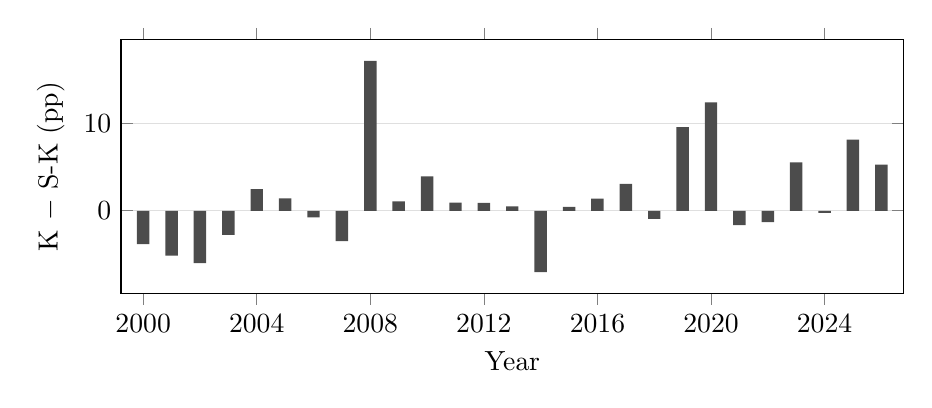
\begin{tikzpicture}
\begin{axis}[ybar, bar width=4.5pt, width=0.95\textwidth, height=4.8cm, xlabel={Year}, ylabel={K $-$ S-K (pp)},
  xtick={2000,2004,2008,2012,2016,2020,2024}, x tick label style={/pgf/number format/1000 sep=},
  ymajorgrids, grid style={gray!25}, enlarge x limits=0.03]
\addplot[fill=black!70, draw=none] coordinates {(2000,-3.82) (2001,-5.13) (2002,-6.01) (2003,-2.76) (2004,2.47) (2005,1.43) (2006,-0.77) (2007,-3.48) (2008,17.17) (2009,1.07) (2010,3.93) (2011,0.94) (2012,0.91) (2013,0.49) (2014,-7.02) (2015,0.44) (2016,1.39) (2017,3.08) (2018,-0.94) (2019,9.59) (2020,12.41) (2021,-1.63) (2022,-1.29) (2023,5.55) (2024,-0.24) (2025,8.15) (2026,5.30)};
\end{axis}
\end{tikzpicture}
\caption{Return of K minus return of its static mix, by calendar year (2000: October--December; 2026:
January--September). Exploratory.}
\label{fig:year}
\end{figure}

The analysis in this subsection was done after the pre-specified tests and is descriptive.

\paragraph{By year.} The largest timing gains (Figure~\ref{fig:year}) are 2008 ($+17.2$), 2020 ($+12.4$), 2019 ($+9.6$), 2025 ($+8.2$); the largest losses
2014 ($-7.0$), 2002 ($-6.0$), 2001 ($-5.1$), 2000 ($-3.8$). 2008 alone contributes $+17.2$ points and 2000--2003 together $-17.7$. Removing October 2007 to
March 2009 from the later period, the Sharpe ratios become $1.22$ for K, $1.10$ for S-K and $1.03$ for the
fund: timing still helps ($+0.11$), by about half as much.

\paragraph{By regime.} Summing K minus S-K over the months in each regime (percentage points), the later period
gives Goldilocks $+17.1$, Disinflation $+23.6$, Stagflation $+12.3$ and Reflation $-2.8$; the
earlier period gives Goldilocks $-12.5$, Disinflation $-5.9$, Stagflation $-0.4$ and Reflation
$+3.9$. K holds 90\% and 80\% of the fund in Goldilocks and Disinflation against $61\%$ for its static mix,
so most of its timing is a bet that these regimes are good for growth stocks. After 2007 they were (the fund
earned $+31.1\%$ and $+25.1\%$ a year in them); from 2000 to 2007 they were not ($-24.3\%$ and
$-8.1\%$). Cutting the fund in Stagflation mattered less than the design of K suggests.

\begin{figure}[htbp]
\centering
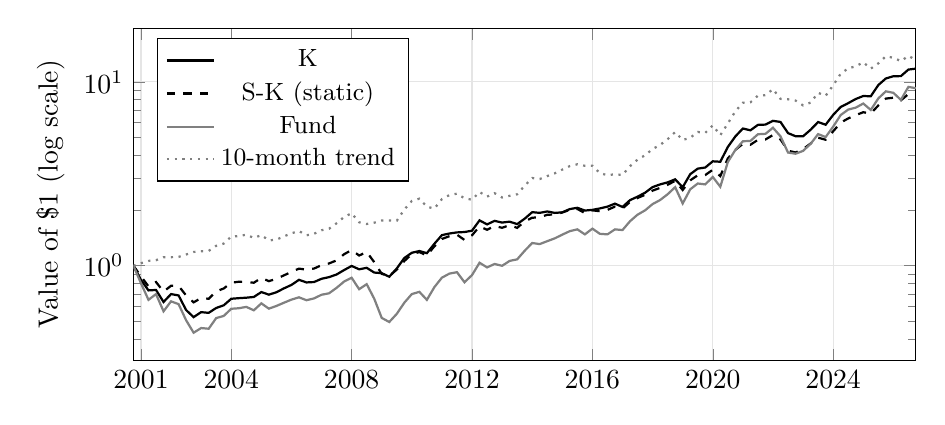
\begin{tikzpicture}
\begin{axis}[width=0.95\textwidth, height=5.8cm, ymode=log, xmin=2000.75, xmax=2026.75,
  xtick={2001,2004,2008,2012,2016,2020,2024}, x tick label style={/pgf/number format/1000 sep=},
  ylabel={Value of \$1 (log scale)}, legend pos=north west, legend style={font=\small}, grid=major, grid style={gray!20}]
\addplot[thick, black] coordinates {(2000.75,1.000) (2001.00,0.837) (2001.25,0.734) (2001.50,0.738) (2001.75,0.635) (2002.00,0.701) (2002.25,0.689) (2002.50,0.574) (2002.75,0.525) (2003.00,0.559) (2003.25,0.554) (2003.50,0.589) (2003.75,0.609) (2004.00,0.661) (2004.25,0.666) (2004.50,0.670) (2004.75,0.676) (2005.00,0.719) (2005.25,0.696) (2005.50,0.717) (2005.75,0.753) (2006.00,0.786) (2006.25,0.838) (2006.50,0.811) (2006.75,0.815) (2007.00,0.849) (2007.25,0.867) (2007.50,0.896) (2007.75,0.947) (2008.00,0.997) (2008.25,0.956) (2008.50,0.974) (2008.75,0.918) (2009.00,0.911) (2009.25,0.871) (2009.50,0.966) (2009.75,1.101) (2010.00,1.176) (2010.25,1.202) (2010.50,1.170) (2010.75,1.317) (2011.00,1.467) (2011.25,1.497) (2011.50,1.518) (2011.75,1.525) (2012.00,1.551) (2012.25,1.765) (2012.50,1.678) (2012.75,1.754) (2013.00,1.717) (2013.25,1.737) (2013.50,1.684) (2013.75,1.803) (2014.00,1.956) (2014.25,1.939) (2014.50,1.974) (2014.75,1.938) (2015.00,1.952) (2015.25,2.033) (2015.50,2.066) (2015.75,1.996) (2016.00,2.013) (2016.25,2.050) (2016.50,2.096) (2016.75,2.176) (2017.00,2.088) (2017.25,2.274) (2017.50,2.375) (2017.75,2.495) (2018.00,2.677) (2018.25,2.770) (2018.50,2.841) (2018.75,2.952) (2019.00,2.673) (2019.25,3.147) (2019.50,3.374) (2019.75,3.422) (2020.00,3.699) (2020.25,3.678) (2020.50,4.426) (2020.75,5.052) (2021.00,5.579) (2021.25,5.453) (2021.50,5.838) (2021.75,5.859) (2022.00,6.141) (2022.25,6.056) (2022.50,5.266) (2022.75,5.064) (2023.00,5.060) (2023.25,5.492) (2023.50,6.050) (2023.75,5.849) (2024.00,6.616) (2024.25,7.302) (2024.50,7.665) (2024.75,8.073) (2025.00,8.383) (2025.25,8.351) (2025.50,9.615) (2025.75,10.439) (2026.00,10.737) (2026.25,10.754) (2026.50,11.671) (2026.75,11.810)}; \addlegendentry{K}
\addplot[thick, black, dashed] coordinates {(2000.75,1.000) (2001.00,0.875) (2001.25,0.772) (2001.50,0.815) (2001.75,0.723) (2002.00,0.778) (2002.25,0.777) (2002.50,0.689) (2002.75,0.632) (2003.00,0.667) (2003.25,0.661) (2003.50,0.725) (2003.75,0.752) (2004.00,0.808) (2004.25,0.818) (2004.50,0.815) (2004.75,0.808) (2005.00,0.858) (2005.25,0.824) (2005.50,0.849) (2005.75,0.886) (2006.00,0.926) (2006.25,0.964) (2006.50,0.952) (2006.75,0.965) (2007.00,1.007) (2007.25,1.029) (2007.50,1.069) (2007.75,1.155) (2008.00,1.217) (2008.25,1.136) (2008.50,1.189) (2008.75,1.046) (2009.00,0.903) (2009.25,0.879) (2009.50,0.952) (2009.75,1.060) (2010.00,1.157) (2010.25,1.186) (2010.50,1.138) (2010.75,1.275) (2011.00,1.398) (2011.25,1.448) (2011.50,1.475) (2011.75,1.381) (2012.00,1.464) (2012.25,1.635) (2012.50,1.569) (2012.75,1.645) (2013.00,1.608) (2013.25,1.663) (2013.50,1.607) (2013.75,1.743) (2014.00,1.824) (2014.25,1.835) (2014.50,1.892) (2014.75,1.902) (2015.00,1.948) (2015.25,2.015) (2015.50,2.036) (2015.75,1.934) (2016.00,2.001) (2016.25,1.979) (2016.50,2.013) (2016.75,2.096) (2017.00,2.047) (2017.25,2.224) (2017.50,2.336) (2017.75,2.432) (2018.00,2.562) (2018.25,2.651) (2018.50,2.756) (2018.75,2.897) (2019.00,2.582) (2019.25,2.913) (2019.50,3.104) (2019.75,3.115) (2020.00,3.326) (2020.25,3.074) (2020.50,3.835) (2020.75,4.272) (2021.00,4.603) (2021.25,4.548) (2021.50,4.842) (2021.75,4.862) (2022.00,5.142) (2022.25,4.861) (2022.50,4.225) (2022.75,4.131) (2023.00,4.303) (2023.25,4.623) (2023.50,4.971) (2023.75,4.846) (2024.00,5.388) (2024.25,6.002) (2024.50,6.332) (2024.75,6.596) (2025.00,6.840) (2025.25,6.733) (2025.50,7.445) (2025.75,8.115) (2026.00,8.204) (2026.25,7.940) (2026.50,8.587) (2026.75,8.588)}; \addlegendentry{S-K (static)}
\addplot[thick, gray] coordinates {(2000.75,1.000) (2001.00,0.803) (2001.25,0.652) (2001.50,0.701) (2001.75,0.565) (2002.00,0.640) (2002.25,0.618) (2002.50,0.505) (2002.75,0.432) (2003.00,0.458) (2003.25,0.454) (2003.50,0.519) (2003.75,0.533) (2004.00,0.583) (2004.25,0.587) (2004.50,0.597) (2004.75,0.572) (2005.00,0.624) (2005.25,0.584) (2005.50,0.604) (2005.75,0.629) (2006.00,0.654) (2006.25,0.673) (2006.50,0.649) (2006.75,0.664) (2007.00,0.695) (2007.25,0.708) (2007.50,0.758) (2007.75,0.820) (2008.00,0.860) (2008.25,0.745) (2008.50,0.794) (2008.75,0.662) (2009.00,0.520) (2009.25,0.494) (2009.50,0.547) (2009.75,0.629) (2010.00,0.701) (2010.25,0.721) (2010.50,0.652) (2010.75,0.765) (2011.00,0.861) (2011.25,0.906) (2011.50,0.922) (2011.75,0.813) (2012.00,0.889) (2012.25,1.038) (2012.50,0.979) (2012.75,1.022) (2013.00,0.999) (2013.25,1.062) (2013.50,1.083) (2013.75,1.206) (2014.00,1.329) (2014.25,1.311) (2014.50,1.360) (2014.75,1.409) (2015.00,1.476) (2015.25,1.542) (2015.50,1.577) (2015.75,1.481) (2016.00,1.591) (2016.25,1.491) (2016.50,1.481) (2016.75,1.577) (2017.00,1.563) (2017.25,1.746) (2017.50,1.895) (2017.75,2.001) (2018.00,2.164) (2018.25,2.277) (2018.50,2.448) (2018.75,2.675) (2019.00,2.180) (2019.25,2.603) (2019.50,2.801) (2019.75,2.770) (2020.00,3.040) (2020.25,2.689) (2020.50,3.665) (2020.75,4.266) (2021.00,4.755) (2021.25,4.774) (2021.50,5.192) (2021.75,5.218) (2022.00,5.633) (2022.25,5.058) (2022.50,4.128) (2022.75,4.067) (2023.00,4.214) (2023.25,4.601) (2023.50,5.201) (2023.75,5.011) (2024.00,5.711) (2024.25,6.604) (2024.50,7.072) (2024.75,7.244) (2025.00,7.629) (2025.25,7.039) (2025.50,8.132) (2025.75,8.888) (2026.00,8.725) (2026.25,7.985) (2026.50,9.395) (2026.75,9.240)}; \addlegendentry{Fund}
\addplot[thick, gray, dotted] coordinates {(2000.75,1.000) (2001.00,1.032) (2001.25,1.062) (2001.50,1.071) (2001.75,1.113) (2002.00,1.113) (2002.25,1.116) (2002.50,1.151) (2002.75,1.188) (2003.00,1.198) (2003.25,1.204) (2003.50,1.283) (2003.75,1.319) (2004.00,1.441) (2004.25,1.450) (2004.50,1.475) (2004.75,1.416) (2005.00,1.467) (2005.25,1.373) (2005.50,1.386) (2005.75,1.444) (2006.00,1.501) (2006.25,1.544) (2006.50,1.464) (2006.75,1.491) (2007.00,1.560) (2007.25,1.589) (2007.50,1.702) (2007.75,1.842) (2008.00,1.930) (2008.25,1.723) (2008.50,1.686) (2008.75,1.714) (2009.00,1.762) (2009.25,1.761) (2009.50,1.757) (2009.75,2.021) (2010.00,2.250) (2010.25,2.316) (2010.50,2.094) (2010.75,2.046) (2011.00,2.303) (2011.25,2.423) (2011.50,2.466) (2011.75,2.326) (2012.00,2.286) (2012.25,2.519) (2012.50,2.375) (2012.75,2.481) (2013.00,2.351) (2013.25,2.400) (2013.50,2.447) (2013.75,2.725) (2014.00,3.001) (2014.25,2.962) (2014.50,3.073) (2014.75,3.182) (2015.00,3.334) (2015.25,3.484) (2015.50,3.563) (2015.75,3.498) (2016.00,3.501) (2016.25,3.187) (2016.50,3.109) (2016.75,3.144) (2017.00,3.117) (2017.25,3.481) (2017.50,3.779) (2017.75,3.990) (2018.00,4.315) (2018.25,4.540) (2018.50,4.881) (2018.75,5.334) (2019.00,4.831) (2019.25,4.966) (2019.50,5.343) (2019.75,5.283) (2020.00,5.799) (2020.25,5.129) (2020.50,5.942) (2020.75,6.916) (2021.00,7.709) (2021.25,7.740) (2021.50,8.418) (2021.75,8.461) (2022.00,9.134) (2022.25,8.085) (2022.50,8.045) (2022.75,7.917) (2023.00,7.450) (2023.25,7.717) (2023.50,8.723) (2023.75,8.405) (2024.00,9.580) (2024.25,11.077) (2024.50,11.861) (2024.75,12.150) (2025.00,12.795) (2025.25,11.807) (2025.50,12.616) (2025.75,13.788) (2026.00,13.536) (2026.25,12.974) (2026.50,13.851) (2026.75,13.166)}; \addlegendentry{10-month trend}
\end{axis}
\end{tikzpicture}
\caption{Growth of \$1, 2000-10 to 2026-09, after costs, quarter-end values.}
\label{fig:wealth}
\end{figure}

\subsection{Costs and implementation}

\begin{table}[htbp]
\centering
\caption{Sharpe ratio and cost drag (bps a year) of K at one, two and five times base costs; Sharpe ratio of S-K
for comparison.}
\label{tab:cost}
\small
\begin{tabular}{@{}lrrrrrr@{}}
\toprule
& \multicolumn{2}{c}{K, 2007--2026} & \multicolumn{2}{c}{K, 2000--2007} & \multicolumn{2}{c}{S-K Sharpe} \\
\cmidrule(lr){2-3}\cmidrule(lr){4-5}\cmidrule(lr){6-7}
Costs & Sharpe & bps/yr & Sharpe & bps/yr & 2007--26 & 2000--07 \\
\midrule
$\times1$ & $1.069$ & $2.8$ & $-0.355$ & $4.0$ & $0.844$ & $-0.180$ \\
$\times2$ & $1.066$ & $5.6$ & $-0.359$ & $8.1$ & $0.844$ & $-0.180$ \\
$\times5$ & $1.059$ & $14.0$ & $-0.369$ & $20.1$ & $0.843$ & $-0.181$ \\
\bottomrule
\end{tabular}
\end{table}

ETF trading costs do not decide anything: K turns over $2.94$ times its value a year, which costs $2.8$
basis points a year at base costs and $14.0$ at five times base (Table~\ref{tab:cost}). Two costs not in
the table matter more. Mutual funds restrict frequent purchases and redemptions, and moving 30--75\% of a
portfolio in and out of a fund several times a year may breach those policies. In a taxable account each cut
realises capital gains. Both favour the static mix, which only rebalances (turnover $0.32$ a year).

%=====================================================================
\section{Implications}

\paragraph{For research on regime allocation.} Build regimes from real-time data; with revised data a third of
the labels in a typical backtest were not knowable, and growth data are the problem. Do not fit allocations to
regime means: a table estimated on 2007--2026 would cut growth equity in Stagflation, one estimated on 1992--2007
would raise it. Show that a rule works in a period that was not used to design it, and separate its timing from
its average allocation.

\paragraph{For the investor.} Holding about 60\% of the fund with gold, short Treasuries, high yield and dollars,
without timing, reduced the worst drawdown in both periods and raised the Sharpe ratio, significantly before
2007 and over 2000--2026 (after 2007 the interval includes zero); this is the robust part.
The timing amounts to holding more growth equity when the classifier says Goldilocks or Disinflation and much
less in Stagflation. It paid off after 2007 and cost money in 2000--2007; adopting it is a bet that the
post-2007 relation continues. A 10-month trend rule, which needs no macro data, was the best strategy in
2000--2007 and matched the overlay's drawdown afterwards.

%=====================================================================
\section{Limitations}

\paragraph{Few episodes.} Each period is dominated by one crash, 2000--2002 and 2008. Bootstrap intervals describe
sampling noise around one history, and the hold-out assets behave like about $1.2$ independent series; no
statistical method creates more crises.

\paragraph{The overlay was designed on 2011--2026.} The later period overlaps the data used to choose K, so its
results there are partly in sample. Only 2000--2007 is fully out of sample, and it is 78 months long.

\paragraph{Proxies.} Before 2007 the sleeves are mutual funds and futures indices. Their tracking errors are small
for Treasuries, gold and the dollar but larger for high yield and commodities (Table~\ref{tab:proxy}).

\paragraph{One growth series, one horizon, one country.} Industrial production covers a shrinking share of the
economy; real-time employment or GDP vintages could give a better growth signal. We test next-month returns
only, and only in the United States.

%=====================================================================
\section{Conclusion}

A growth--inflation classifier run on the data available at the time differs from the backtested version in a
third of months and does not forecast next month's returns of any of twelve asset classes after accounting for
multiple tests. For growth equities the effect of Stagflation reverses sign around 2007. A regime overlay for a
concentrated growth fund, tested under a frozen specification, improves risk-adjusted returns in 2007--2026
(partly in sample) and mainly through the 2008 crisis; its timing is negative, though not significantly, in
2000--2007 for the fund and for ten other equity assets, while its
average allocation reduces the drawdown in both periods and raises the Sharpe ratio over the whole sample. A standard predictive regression on the same signals has no out-of-sample skill, and the
stock--bond correlation does not explain the change.
The defensible recommendation is static diversification, possibly with a simple trend rule; regime timing is a
view on the current era, not a backtested improvement.

\appendix
\section{Proxies before ETF inception}
\label{app:proxy}

Each ETF is replaced before its first full month by a long-history series. For each pair the version (with or
without adding the T-bill rate, for futures-based indices) with the lower tracking error on the 2007--2026
overlap was chosen before any backtest.

\begin{table}[htbp]
\centering
\caption{Proxies compared with the ETF on 2007-05 to 2026-09: correlation of monthly returns, tracking error,
and ETF minus proxy average return per year.}
\label{tab:proxy}
\small
\begin{tabular}{@{}llrrr@{}}
\toprule
ETF & Proxy & Corr. & TE & ETF $-$ proxy \\
\midrule
HYG (High yield) & VWEHX & $0.906$ & $4.5\%$ & $-0.40\%$ \\
SHY (1--3y Treasuries) & VFISX & $0.968$ & $0.5\%$ & $-0.11\%$ \\
IEF (7--10y Treasuries) & VFITX & $0.981$ & $2.3\%$ & $+0.27\%$ \\
TLT (20y+ Treasuries) & VUSTX & $0.991$ & $2.3\%$ & $+0.02\%$ \\
GLD (Gold) & GC=F & $0.992$ & $2.3\%$ & $-0.37\%$ \\
DBC (Commodities) & \^{}SPGSCI + T-bill & $0.956$ & $7.3\%$ & $-2.27\%$ \\
UUP (US dollar) & DX-Y.NYB + T-bill & $0.994$ & $0.9\%$ & $-0.79\%$ \\
\bottomrule
\end{tabular}
\end{table}

\begin{thebibliography}{99}
\bibitem[Ang and Bekaert(2002)]{ang2002} Ang, A. and Bekaert, G. (2002). International asset allocation with regime shifts. \emph{Review of Financial Studies}, 15(4), 1137--1187.
\bibitem[Bailey and L\'opez de Prado(2014)]{bailey2014} Bailey, D.~H. and L\'opez de Prado, M. (2014). The deflated Sharpe ratio: correcting for selection bias, backtest overfitting, and non-normality. \emph{Journal of Portfolio Management}, 40(5), 94--107.
\bibitem[Campbell et al.(2020)]{campbell2020} Campbell, J.~Y., Pflueger, C. and Viceira, L.~M. (2020). Macroeconomic drivers of bond and equity risks. \emph{Journal of Political Economy}, 128(8), 3148--3185.
\bibitem[Croushore and Stark(2001)]{croushore2001} Croushore, D. and Stark, T. (2001). A real-time data set for macroeconomists. \emph{Journal of Econometrics}, 105(1), 111--130.
\bibitem[Faber(2007)]{faber2007} Faber, M.~T. (2007). A quantitative approach to tactical asset allocation. \emph{Journal of Wealth Management}, 9(4), 69--79.
\bibitem[Harvey et al.(2016)]{harvey2016} Harvey, C.~R., Liu, Y. and Zhu, H. (2016). \ldots and the cross-section of expected returns. \emph{Review of Financial Studies}, 29(1), 5--68.
\bibitem[Ilmanen(2011)]{ilmanen2011} Ilmanen, A. (2011). \emph{Expected Returns: An Investor's Guide to Harvesting Market Rewards}. Wiley.
\bibitem[Ledoit and Wolf(2008)]{ledoit2008} Ledoit, O. and Wolf, M. (2008). Robust performance hypothesis testing with the Sharpe ratio. \emph{Journal of Empirical Finance}, 15(5), 850--859.
\bibitem[Moreira and Muir(2017)]{moreira2017} Moreira, A. and Muir, T. (2017). Volatility-managed portfolios. \emph{Journal of Finance}, 72(4), 1611--1644.
\bibitem[Moskowitz et al.(2012)]{moskowitz2012} Moskowitz, T.~J., Ooi, Y.~H. and Pedersen, L.~H. (2012). Time series momentum. \emph{Journal of Financial Economics}, 104(2), 228--250.
\bibitem[Newey and West(1987)]{newey1987} Newey, W.~K. and West, K.~D. (1987). A simple, positive semi-definite, heteroskedasticity and autocorrelation consistent covariance matrix. \emph{Econometrica}, 55(3), 703--708.
\bibitem[Orphanides(2001)]{orphanides2001} Orphanides, A. (2001). Monetary policy rules based on real-time data. \emph{American Economic Review}, 91(4), 964--985.
\bibitem[Politis and Romano(1994)]{politis1994} Politis, D.~N. and Romano, J.~P. (1994). The stationary bootstrap. \emph{Journal of the American Statistical Association}, 89(428), 1303--1313.
\bibitem[Welch and Goyal(2008)]{welch2008} Welch, I. and Goyal, A. (2008). A comprehensive look at the empirical performance of equity premium prediction. \emph{Review of Financial Studies}, 21(4), 1455--1508.
\end{thebibliography}

\end{document}
